\scanpage{29}
$\unsure{\gamma}$ commute aux Inf finis ?

\[
\begin{aligned}
\deleted{\unsure{\alpha(}}\qquad \unsure{\gamma|\alpha}(X\times Y)&=\alpha(X)\beta(Y)=1_O\\
\gamma(W\cap W')&=\operatorname*{Sup}_{U\times V\subset W\cap W'}\alpha(U)\cap\beta(\unsure{W|V})
=\operatorname*{Sup}_{\substack{U\times V\subset W\\ U'\times V'\subset W'}}
 \underbrace{\alpha(U\cap U')\cap\beta(V\cap V')}_{\underbrace{\alpha(U)\beta(V)}\quad\underbrace{\alpha(U')\beta(V')}}\\
&=\operatorname*{Sup}_{U\times V\subset W}\alpha(U)\beta(V)\ \wedge\operatorname*{Sup}_{U'\times V'\subset W'}\alpha(U')\beta(V')\\
&=\unsure{\gamma|\mathcal R}(W)\cap\gamma(W')
\end{aligned}
\]

\figure{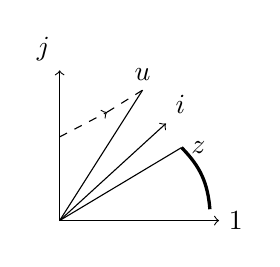
\begin{tikzpicture}[scale=.9]
\draw[->] (0,0)--(2.25,0) node[right] {$1$};
\draw[->] (0,0)--(0,2.12) node[above left] {$j$};
\draw[->] (0,0)--(1.50,1.37) node[above right] {$i$};
\draw (0,0)--(1.72,1.03) node[right] {$z$};
\draw[very thick] (1.72,1.03) to[bend left=20] (2.12,.16);
\draw (0,0)--(1.17,1.84) node[above] {$u$};
\draw[dashed,->] (0,1.18)--(.67,1.53);
\draw[dashed] (.67,1.53)--(1.17,1.84);
\end{tikzpicture}}

\[
1,\ z=e^{i\theta}=\cos\theta+i\sin\theta,\quad u=a+bi+cj
\]

\[
\begin{aligned}
&\deleted{\sin\unsure{\frac{\theta}{2}|\theta}=2\sin\frac{\theta}{2}\cos\frac{\theta}{2})}\\
&\deleted{\cos\theta=\cos^2\frac{\theta}{2}-\sin^2\frac{\theta}{2}}\\
&\deleted{\cot\theta=\tfrac12(}
\end{aligned}
\]

\[
\left\{\begin{aligned}a^2+b^2+c^2&=1\\a&=\cos\theta\end{aligned}\right.
\qquad
\deleted{\left\{\cos^2\theta+b^2+c^2=1\right.}
\]
\[
 a\cos\theta+b\sin\theta=\cos\theta
\]

\[
\begin{aligned}
b&=\unsure{\cot}\theta-\cos\theta\cot\theta=\cot\theta(1-\cos\theta)=2\cot\theta\sin^2\tfrac\theta2\\
c^2&=1-a^2-b^2\\
&\deleted{=\sin^2\theta-\unsure{4\cot^2\theta\sin^2(\theta/2)}}\\
&=\sin^2\theta-4\cot^2\theta\sin^4\tfrac\theta2
\end{aligned}
\]

\figure{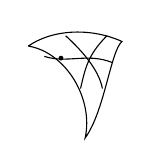
\begin{tikzpicture}[scale=.73]
\draw (0,1.6) .. controls (.46,1.91) and (1.12,1.91) .. (1.63,1.68)
 .. controls (1.43,1.50) and (1.33,.47) .. (.99,0)
 .. controls (1.14,.68) and (.66,1.49) .. (0,1.6);
\draw (.28,1.42) .. controls (.69,1.29) and (1.03,1.49) .. (1.47,1.31);
\draw (.65,1.78) .. controls (.88,1.57) and (1.23,1.21) .. (1.29,.86);
\draw (1.37,1.78) .. controls (1.03,1.44) and (.99,1.20) .. (.91,.86);
\fill (.57,1.39) circle (.042);
\end{tikzpicture}}

% A large X crosses the central working and continues into the Hom calculation below.
\[
\begin{aligned}
&\deleted{(u+v+w)^2=\unsure{u^2}+v^2\unsure{+}w^2+2(uv+vw+wu)}\\
&\deleted{\phantom{(u+v+w)^2}=3+6\cos3\theta=3(1+2\cos3\theta)}
\end{aligned}
\]

\[
\deleted{\left\{\begin{aligned}u+v+w&=\sqrt{3(1+2\cos3\theta)}\,a\\uv&=\cos\theta\\vw&=\cos\theta\\wu&=\cos\theta\end{aligned}\right.}
\]

\[
\begin{aligned}
\cos3\theta&=\cos\theta\cos2\theta-\sin\theta\sin2\theta\\
&=\cos\theta(\cos^2\theta-\sin^2\theta)\\
&\qquad-2\sin^2\theta\cos\theta\\
&=\cos^3\theta-3\sin^2\theta\cos\theta\ \deleted{\unsure{(=\cos\theta-4\mathrm{si}}}\\
&\deleted{=\cos\theta-4\sin^2\theta\cos\theta}\\
&\deleted{3+6\cos3\theta=3+6\cos^3\theta}\\
&\deleted{3+6\cos\theta-24\sin^2\theta\cos\theta}\\
&\cos\theta(1-\underbrace{4\sin^2\theta}_{\deleted{\unsure{\sin^22\theta}}})\\
&\deleted{\unsure{\cos\theta(1-2\sin^2\theta)}}
\end{aligned}
\]

$X\times Y$

\diagram{\begin{tikzcd}[ampersand replacement=\&,column sep=large]
O_X\arrow[r,"{U\mapsto(U,Y)}"]\&O_X\times O_Y\arrow[r,"{(U,V)\mapsto U\times V}"']\&\underline O_{X\times Y}\\
O_Y\arrow[r,"{V\mapsto(X,V)}"']\&{}\&
\end{tikzcd}}

\margin{$\mathrm{Hom}'$: \deleted{\unsure{u}}\inserted{croiss.} commutant aux Sup, quelcon. et Inf finis ;}

\[
\deleted{\operatorname{Hom}'(\underline O_{X\times Y},O)\xrightarrow{u\longmapsto\alpha,\beta}\operatorname{Hom}'(O_X,O)\times\operatorname{Hom}'(O_Y,O)}
\]

\margin{$O$ muni \deleted{Sup} et Inf quelcon, et Inf distributif pour Sup quel}

\deleted{injectif car $u\in\operatorname{Hom}'(O_{X\times Y},O)$ est connu si on connaît ses $u(U\times V)$\inserted{$=\alpha(U)\cap\beta(V)$}, puisque \uline{tout} $W\in O_{X\times Y}$ est Sup de tels $U\times V$.}

Est-ce bijectif ? soit $\alpha:O_X\longrightarrow O$, $\beta:O_Y\longrightarrow O$
Construisons $\gamma:O_{X\times Y}\mathbin{\unsure{-|\to}}O$

posons

\[
\gamma(W)=\operatorname*{Sup}_{\substack{U\in O_X\\V\in O_Y\\U\times V\subset W}}\alpha(\unsure{U|X})\cap\beta(V)
\]

\margin{SPG $\begin{gathered}X\ne\varnothing\\Y\ne\varnothing\end{gathered}$}

C'est une application \uline{croissante} $O_{X\times Y}\longrightarrow O$

\margin{$X'\in\mathrm{Ouv}(X)$}

$\alpha(X'\times Y)=\ ?$ noter que si $Y\ne\varnothing$, alors $U\times V\subset X'\times Y'$ sss $U\subset X'$
donc le Sup est $\deleted{\unsure{\mathrm{Sup}|\text{égal}}}\alpha(X')\cap\beta(Y)=\alpha(X')$
% archive sheet number: 28
